\section{Uvod u web}
\label{sec:uvodweb}
Danas, ne možemo zamisliti korišćenje računara bez veza ka drugim računarima. Izgradnja računarskih mreža, a posebno sa nastankom i razvojem Interneta i njegovih servisa poput Veba, dovele su do porasta broja korisnika računara i promene uloga računara u odnosu na ranije. Pojava savremenih računarskih mreža smatra se revolucionarnom poput pojave parne mašine u $18.$ veku. Svake godine uvećava se broj umreženih računara, a sa tim brojem raste i broj usluga koje nam mrežno okruženje nudi. Neke od osnovnih primera upotreba računarskih mreža obuhvataju:
\begin{itemize}
\item poslovna: elektronska pošta, razmena datoteka, deljeni štampači, ...
\item kućna: filmovi, muzika, igrice, vesti, audio i video komunikacija, razmena poruka, elektronska kupovina,...
\item mobilne: pozivi, SMS, igrice, mape, pristup informacijama
\end{itemize}

\subsection{Uloga računarskih mreža}
U osnovne uloge računarskih mreža ubrajamo:
\begin{enumerate}

\item komunikaciju - uz pomoć računara ljudi razmenjuju poruke, video pozive, mejlove, ćaskanja (eng. chat), video konferencije, itd.
\item deljenje informacija i podataka - ako postoji mrežno okruženje u kom su računari povezani, tada je moguće pristupiti informacijama na drugim računarima u okviru mreže. Podatke prenosimo na više načina, kao što su preuzimanje datoteka, prenos informacija u okviru lokalnih mreža (obično u okviru jedne kompanije), kao i u okviru globalne svetske mreže. Internet i veb se smatraju glavnim izvorima informacija. 
\item deljenje softvera - korisnici povezani u mrežu mogu koristiti mnoge usluge koje im pruža softver koji radi na računarima u okviru mreže. Neke od usluga su kupovina i rezervacija karata preko interneta, ili izvršavanje softvera koji je distribuiran i paralelizovan na više povezanih računara, čime se može ubrzati izvršavanje.
\item deljenje hardverskih resursa - obezbeđuje zajedničko korišćenje hardvera, poput štampača, skenera i ostalih. Često se ovakav pristup koristi u kompanijama.
\end{enumerate} 

Računarski resursi u mreži mogu biti raspoređeni na različite načine, tako da obezbeđuju različite načine izvršavanja poslova. Neki od najčešćih su:
\begin{itemize}
\item Centralizovana obrada - svi poslovi se izvršavaju na jednom centralnom računaru, dok se ostali uređaji u mreži koriste samo kao terminali za unos podataka i prikaz rezultata. Ovakavim načinom rada odlikovale su se rane računarske mreže.
\item Klijent-server okruženje - jedan računar ima ulogu servera na kome se nalaze
podaci i aplikativni softver, koji se stavljaju na raspolaganje klijentima. Serveri su obično moćniji računari od klijenata(mada ne mora uvek biti tako) i na njima se obavljaju zadaci koji zahtevaju više resursa. U današnjem kontekstu, stroga podela na klijentski i serverski računar više nije tako aktuelna. Najčešće govorimo o tome da je jedan računar istovremeno i klijent i server u zavisnosti od zadataka koji su mu zadati. Na primer, isti računar može istovremeno pokretati i Veb server i klijent za elektronsku poštu, čime mu je data i uloga servera i uloga klijenta.
na njihov zahtev. 
\item Mreža ravnopravnih računara (eng. peer-to-peer - $P2P$) - računari direktno komuniciraju deleći podatke i opremu. Sve se češće ovakve mreže koriste za masovnu razmenu velikih količina podataka (npr. torenti - Bittorrent).
\end{itemize}
\begin{figure}[h!]
\begin{center}
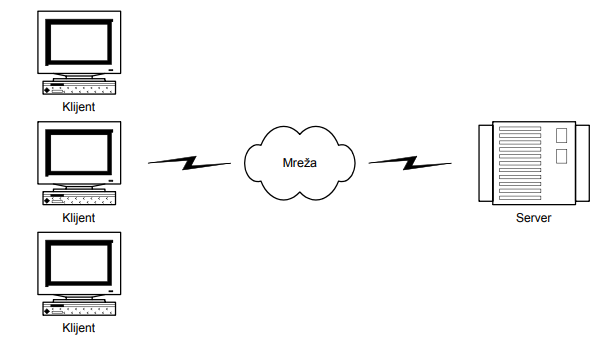
\includegraphics[scale=0.5]{pictures/KS.png}
\end{center}
\caption{Prikaz klijent-server arhitekture.}
\label{fig:KS}
\end{figure}

\subsection{Komponente računarskih mreža}
Pre nego što uđemo u detaljniji opis elemenata koji čine jednu računarsku mrežu, trebalo bi da damo formalnu definiciju šta je računarska mreža. Naime, računarska mreža je sistem koji se sastoji iz skupa hardverskih uređaja koji su međusobno povezani komunikacijskom opremom i koji je snabdeven odgovarajućim kontrolnim softverom kojim se ostvaruje kontrola funkcionisanja sistema tako da je moguć prenos podataka između povezanih uređaja. Neke od osnovnih komponenti računarskih mreža su, dakle:
\begin{itemize}
\item mrežni hardver, 
\item komunikacioni kanali i 
\item mrežni softver.
\end{itemize}

\begin{figure}[h!]
\begin{center}
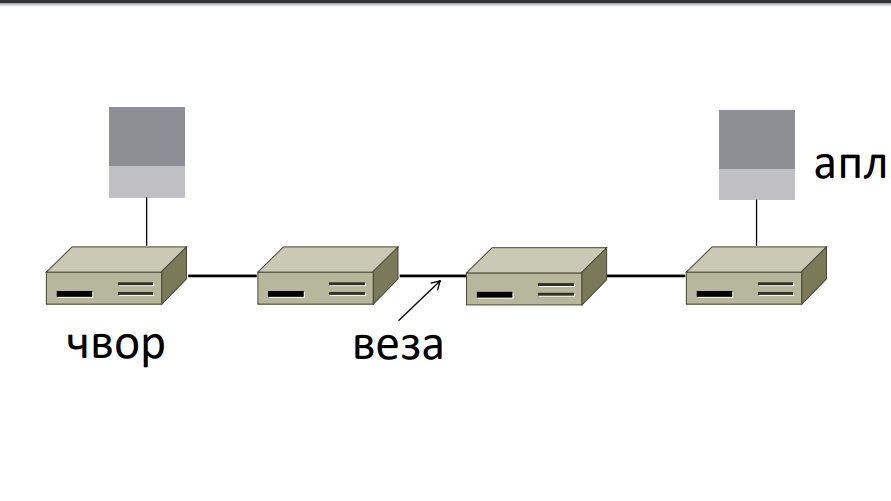
\includegraphics[scale=0.5]{pictures/PrMr.png}
\end{center}
\caption{Prikaz mreže.}
\label{fig:PrMr}
\end{figure}

\subsubsection{Mrežni hardver}
Tradicionalno, podrazumeva se povezivanje računara u okviru mreže, ili uz dodatak nekih pomoćnih uređaja poput štampača, skenera itd., kako bi se mogli deljeno koristiti. Međutim, u poslednje vreme, granica između klasičnih računara i digitalnih uređaja specijalizovane namene se briše i sve češće se u oviru mreže mogu povezati i PDA uređaji, mobilni telefoni, foto aparati, kamere i ostali. Aktivno se radi i na razvoju automobila, frižidera i ostalih mnogobrojnih uređaja kako bi se uključili u mrežu i kako bi se time omogućilo upravljanje istima na daljinu.\\\\
Da bismo neki uređaj mogli da ubacimo u mrežu, neophodno je da sadrži određene hardverske komponente koje bi mu to omogućile. Deo hardvera koji je namenjen za umrežavanje i spada u komunikacionu opremu je mrežna kartica ili mrežni adapter (eng. NIC - network interface card) koja omogućava fizički pristup mreži. Svaka mrežna kartica ima svoju jedinstvenu fizičku (MAC) adresu, kojom se uređaj jedinstveno identifikuje prilikom komunikacije. Neke mrežne kartice obezbeđuju pristup žičanim, a neke druge bežičnim komunikacionim kanalima. Osim mrežnih kartica za umrežavanje se koriste i modemi (telefonski, kablovski), kao i još neki uređaji o kojima neće biti reči. 
\begin{figure}[h!]
\begin{center}
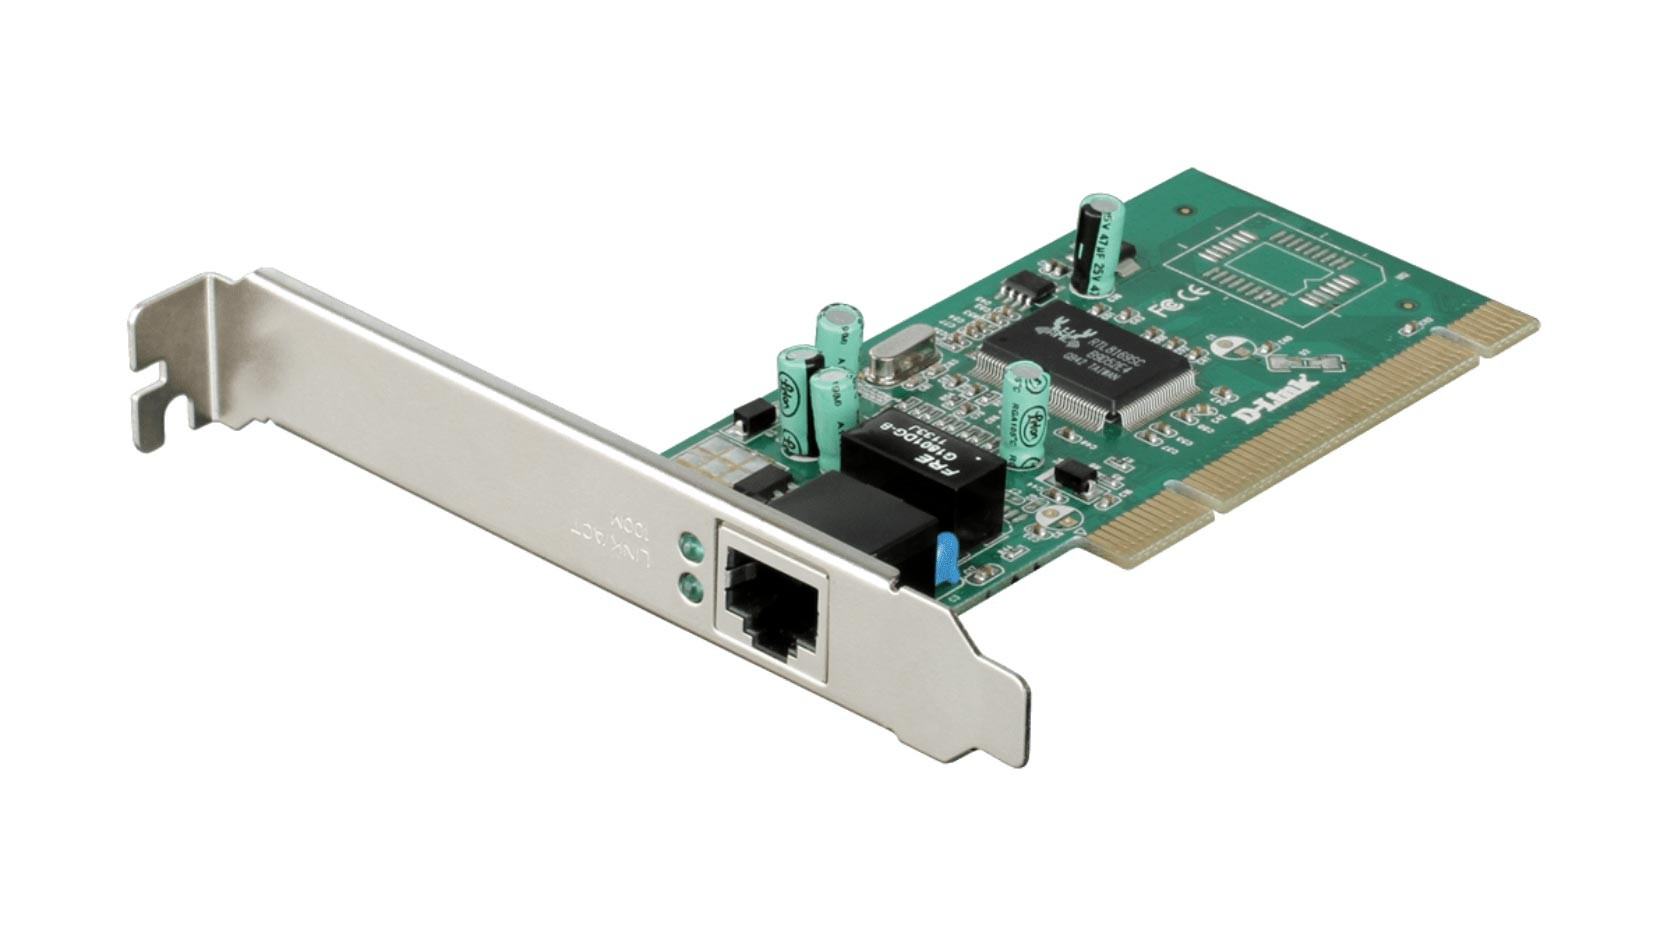
\includegraphics[scale=0.25]{pictures/mreznakartica.jpg}
\end{center}
\caption{Prikaz mrežne kartice.}
\label{fig:mk}
\end{figure}


\subsubsection{Komunikacioni kanali}
Da bi mreža funkcionisala i da bi kroz nju bilo moguće preneti podatke, uređaji koji se nalaze u mreži moraju biti povezani međusobno uz pomoć žičanih ili bežičnih prenosnih sistema, koji predstavljaju komunikacione kanale. Osnovna mera kvaliteta komunikacionog kanala je brzina prenosa koja se meri u bitovima po sekundi (bit/s). Ova mera označava broj bitova koji se mogu preneti kroz komunikacioni kanal u jednoj sekundi. Ako bismo posmatrali aktuelne tehnologije prenosa podataka, najčešće se koriste megabiti ( milion bita) u sekundi - Mbps, ili gigabiti (milijarda bita) u sekundi - Gbps. Brzina prenosa predstavlja fizičku karakteristiku komunikacionog kanala i zavisi od frekvencijskog opsega (eng. bandwidth) koji se može propustiti kroz kanala bez gubitka signala. Na slici \ref{fig:opseg} prikayan je raspon frekvencija za razne prenosne tehnologije. \\\\

\begin{figure}[h!]
\begin{center}
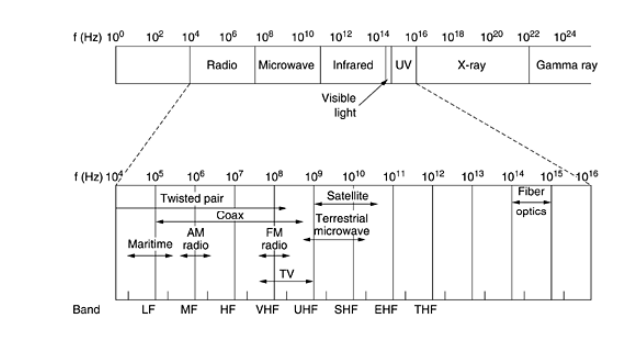
\includegraphics[scale=0.7]{pictures/bandw.png}
\end{center}
\caption{Prikaz frekvencijskih opsega za razne prenosne tehnologije.}
\label{fig:opseg}
\end{figure}

Komunikacione kanale možemo podeliti u dve grupe prema tipu prenosa informacija:
\begin{enumerate}
\item Žičane  
\item Bežične 
\end{enumerate}

\subparagraph{Žičane komunikacije} 
\subparagraph{Parice}(eng. twisted-pair wire) - Najkorišćeniji način komunikacije. Uređaji se povezuju korišćenjem uvijenih uparenih izolovanih bakarnih žica. Žice se uparuju i uvijaju kako bi se smanjile smetnje u komunikaciji. Brzina prenosa kroz ovakav medijum obično varira od $2Mbps$ do $100Mbps$.
\begin{figure}[h!]
\begin{center}
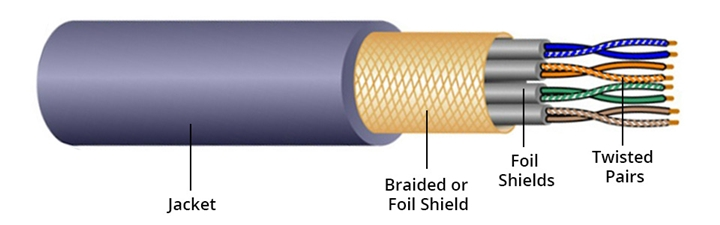
\includegraphics[scale=0.5]{pictures/twpw.jpg}
\end{center}
\caption{Prikaz parice.}
\label{fig:twpw}
\end{figure}

\subparagraph{Koaksijalni kablovi} svoju upotrebu najčešće nalaze u televizijskim kablovskim sistemima, a koriste se i u lokalnim mrežama u kompanijama. Kablovi se sastoje od centralne bakarne ili aluminijumske žice obmotane savitljivim slojem izolacije, oko kog je obmotan provodni sloj tankih žica, a potom je sve to izolovano. Ovaj tip kablova omogućava brzinu prenosa do $200Mbps$ (nekad čak i do $500Mbps$), uz manju osetljivost na elektromagnetne smetnje. 

\begin{figure}[h!]
\begin{center}
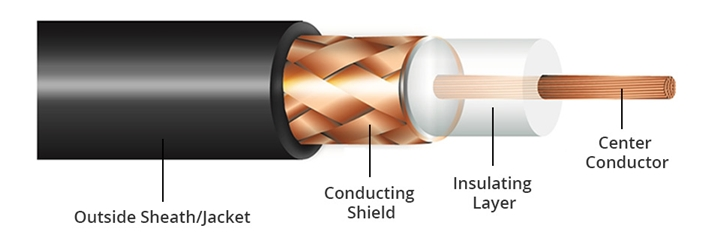
\includegraphics[scale=0.5]{pictures/coax.jpg}
\end{center}
\caption{Prikaz koaksijalnog kabla.}
\label{fig:coax}
\end{figure}

\subparagraph{Optički kablovi}- prave se od velikog broja (reda veličine nekoliko stotina ili hiljada) veoma tankih staklenih vlakana. Podaci se prenose svetlosnim talasima uz pomoć malog laserskog uređaja. Na ovaj tip kablova elektromagnetne smetnje nemaju uticaja. Najveći nedostatak ovakvih kablova je cena, izuzetno su skupi i komplikovani za komunikaciju, pa se uglavnom koriste za osovinski deo mreže, na koji se potom drugim vrstama kablova povezuju pojedinačni uređaji. Brzina ovih uređaja predstavlja njihovu najveću prednost. Naime, brzina ovih uređaja može ići i do nekoliko triliona bita u sekundi. Najčešće se koriste za mreže sa brzinama do $10 Gbps$.
\begin{figure}[h!]
\begin{center}
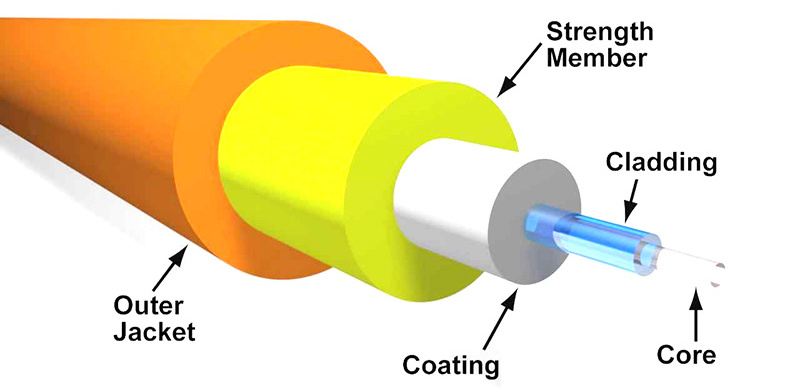
\includegraphics[scale=0.5]{pictures/optical.jpg}
\end{center}
\caption{Prikaz optičkog kabla.}
\label{fig:optical}
\end{figure}

\subparagraph{Bežične komunikacije}
Bežična komunikacija, kao što i samo ime sugeriše, ne koristi kablove za prenos podataka. Ovakav vid komunikacije poseban značaj nalazi kod prenosivih računara, mobilnih telefona ili dosta udaljenih lokacija do kojih bi bilo jako skupo, ako ne i nemoguće, sprovesti kablovsku mrežu. Umesto kablova ove mreže koriste radio talase, mikro talase i infracrvene zrake. Podaci se prenose moduliranjem amplitude, frekvencije ili faze talasa. Neke od danas najkorišćenijih tehnologija su: 
\begin{itemize}
\item Bluetooth - koristi se za veoma male razdaljine (do $10$ ili do $100$ metara. Brzina prenosa je do $3Mbps$. Bluetooth tehnologija koristi radio talase i može da prođe i kroz čvrste prepreke. Koristi se najčešće za komunikaciju računara sa periferjskim uređajima, kao i u mobilnoj telefoniji.
\item Bežični LAN - Wireless LAN (WLAN, WiFi) je tehnologija koja korsti radio talase za bežičnu komunikaciju više uređaja na ograničenim rastojanjima (nekoliko desetina ili stotina metara). Brzina prenosa ide od $10Mbps$ do $50Mbps$ ( u skorije vreme može ići i do $600Mbps$). Najrašireniji standard za ovaj vid komunikacije je IEEE $802.11$, o kome će kasnije biti više reči. 
\item Ćelijski sistemi - Način prenosa je sličan onom koji se koristi u mobilnoj telefoniji. Za komunikaciju se koriste radio talasi i sistemi antena koji pokrivaju određenu geografsku oblast, pri čemu se signal do cilja prenosi preko niza antena. 
\item Zemaljski mikrotalasi - koriste antensku mrežu na Zemlji, a za komunikaciju koriste mikrotalase niske frekvencije koji zahtevaju da antene budu optički vidljive, pa se iste smeštaju na visoke tačke. 
\item Komunikacioni sateliti - koriste mikrotalase za komunikaciju tako što se prenos između dve tačke koje nemaju optičku vidljivost ostvaruje poprečnom komunikacijom preko satelita koji se nalaze u orbiti. Na ovaj način se prenose televizijski i telefonijski signal. Brzina komunikacije je dosta mala $100Mbps$.
\end{itemize}

\subsubsection{Mrežni softver}
Mrežna infrastruktura sama po sebi ne služi ničemu bez mrežnog softvera. Uloga mrežnog softvera je da obezbedi korisniku mrežnu komunikaciju. Na primer, programer pregledača Veba, ne treba da misli o tome kako će pregledač primiti informacije, već treba da se fokusira samo na aspekte značajne za njegovu konkretnu aplikaciju, a sve ostale detalje prepusti nižem sloju mrežnog softvera.

Mrežni softver, najgrublje, može da se podeli na dva nivoa:
\begin{itemize}
\item niskog nivoa - mrežni softver koji omogućuje korišćenje različitih mrežnih uređaja, poput mrežnih kartica, modema, itd. Ovaj softver se nalazi u jezgru operativnog sistema i u obliku upravljača perifernim uređajima, takoznavnih drajvera (eng. driver). On upravlja računarskim hardverom i komunikacijskom opremom. Korisnik nikad ne koristi ovaj softver direktno, a često nije ni svestan njegovog postojanja 
\item visokog nivoa.
\end{itemize}

\subsection{Literatura}
Čitanje literature predstavlja neizostavan deo gradiva, kako naredni izvori predstavljaju odlican izvor informacija, na vama je da ih procitate:
\begin{itemize}
\item Predrag Janičić, Programiranje 1, Matematički fakultet, glava 1
\item Filip Marić, Uvod u web i internet tehnologije, Matematički fakultet, glave 1 i 2
\item Ajzenhamer Nikola, Bukurov Anja, Stanković Vojislav, Programiranje za Veb skripta, glave 1,2 i 3
\end{itemize}
\newpage